Wraz z instalacją Ubuntu na twoim dysku twardym znalazła się cała gama oprogramowania --- pakiet biurowy, przeglądarka internetowa, odtwarzacze multimediów itd. Jednak zapewne chciałbyś zainstalować więcej programów, bardziej odpowiadających twoim potrzebom. W tym rozdziale przedstawione zostaną sposoby instalacji programów w systemie Ubuntu.

W systemach Linuksowych (jakim jest Ubuntu) instalacja programów przebiega nieco inaczej niż gdzie indziej a jednocześnie bardzo podobnie. Jak to możliwe? Bardzo prosto. Zapewne znane Tobie jest pojęcie ,,Sklepu z Oprogramowaniem". Apple ma swój ,,App Store'', Google ma swoje ,,Play''. Są to stosunkowo nowe metody instalacji oprogramowania, które upowszechniły się w przeciągu ostatnich lat. Nawet Microsoft w najnowszych wydaniach swojego systemu Windows promuje instalacje softu przez wbudowany sklep zamiast ręcznego przeszukiwania sieci, ściągania instalatorów, skanowania ich antywirusem i instalowania w systemie.

Takie sklepy z oprogramowaniem istnieją w systemach linuksowych od zarania dziejów, przy czym tutaj nazywają się \textcolor{ubuntu_orange}{repozytoriami}. Repozytorium jest serwerem, na którym opiekunowie danej dystrybucji Linuksa (np. firma Canonical jest opiekunem Ubuntu) przechowują paczki z programami. Użytkownik, chcąc zainstalować jakiś program (np. przeglądarkę internetową Firefox) uruchamia program zwany \textcolor{ubuntu_orange}{menadżerem pakietów}, wyszukuje w nim interesujący go program i instaluje. Nic więcej go nie interesuje --- menadżer pakietów sam ściągnie paczkę z programem, pobierze wszystkie zależności (programy niezbędne do funkcjonowania instalowanego programu) i zainstaluje soft w systemie. Kiedy w repozytoriach program zostanie zaktualizowany to użytkownik zostanie o tym powiadomiony a menadżer pakietów dokona aktualizacji.

W przeciwieństwie do sklepów z oprogramowaniem, system repozytoriów przechowuje nie tylko programy użytkowe, ale też składniki systemu operacyjnego, sterowniki, dokumentację, pliki pomocy, paczki z tematami graficznymi i ikonami oraz wiele innych. Użytkownik nie jest też ograniczony tylko i wyłącznie do repozytoriów oferowanych przez opiekunów dystrybucji i swobodnie może łączyć się z innymi serwerami w celu poszerzenia oferty oprogramowania. W Ubuntu istnieje cały ekosystem repozytoriów PPA (\textit{Personal Package Archive}), które kilkoma kliknięciami można dodać do systemu. Deweloperzy różnych aplikacji za pośrednictwem PPA dostarczają użytkownikom oprogramowanie, które nie znalazło się w repozytoriach oferowanych przez Canonical.

Podstawową jednostką w repozytorium jest paczka. Paczka jest skompresowanym archiwum zawierającym wszystkie pliki programu (czyli soft oraz dodatki: dokumentację, ikony, grafiki, dźwięki i inne) a także informacje co i gdzie ma zostać wypakowane.

\subsubsection{Centrum Oprogramowania Ubuntu}
\textcolor{ubuntu_orange}{Centrum Oprogramowania Ubuntu} jest programem służącym do zarządzania zainstalowanymi aplikacjami. W przeciwieństwie do bardziej rozbudowanej klasy programów zwanych Menadżerami pakietów, Centrum Oprogramowania jest swego rodzaju sklepem z aplikacjami. Znajdziesz tutaj gotowe instalatory programów dostępnych w podstawowych repozytoriach a także programy płatne. Z drugiej strony nie ma tutaj pakietów z podstawowymi składnikami systemu.

\begin{center}
	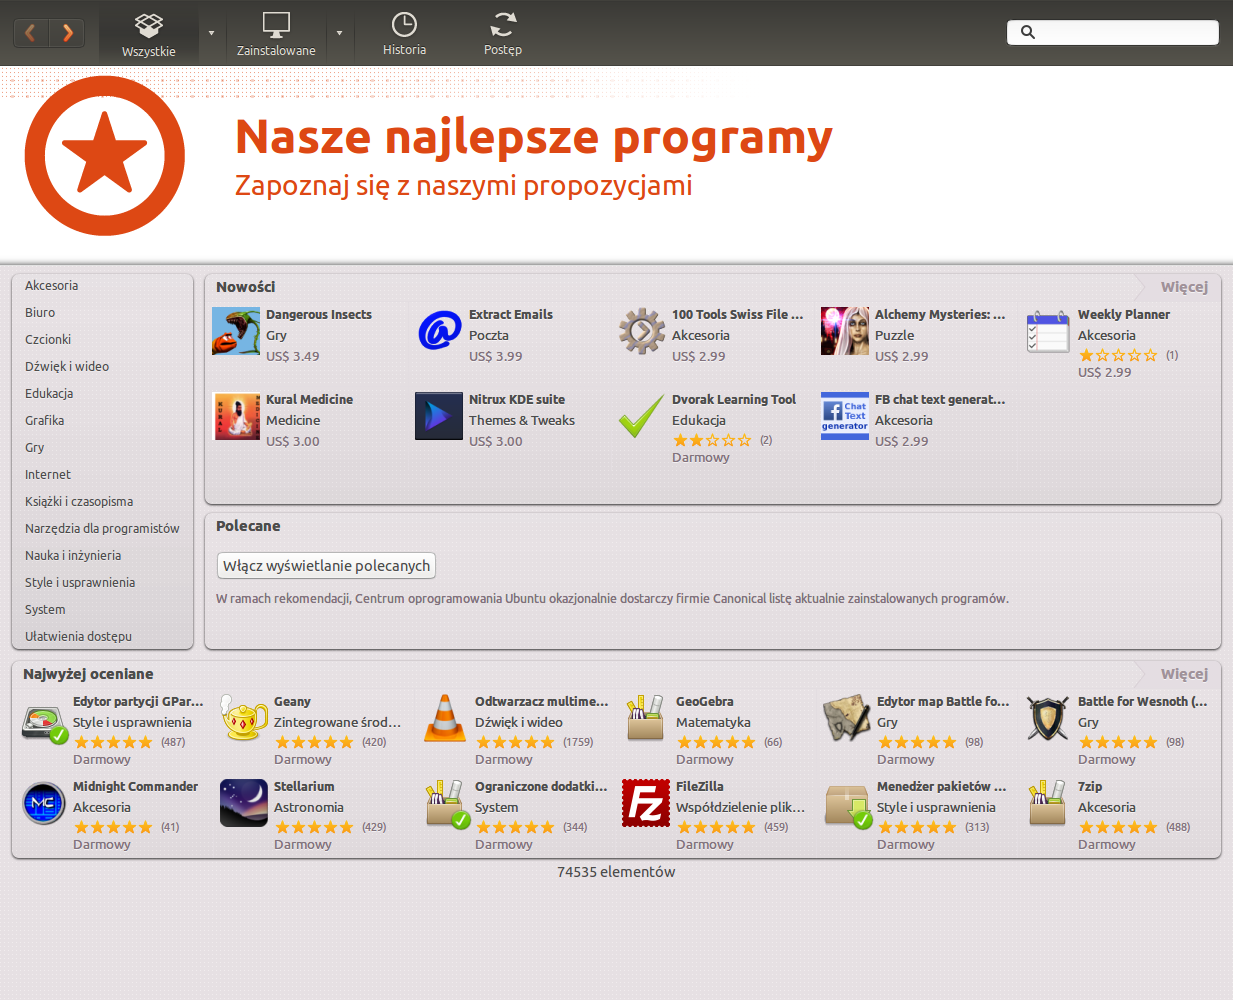
\includegraphics[width=\linewidth]{images/programy_centrum.png}
\end{center} 

W prawym górnym rogu znajduje się pole, w którym możesz wpisać nazwę szukanego programu (lub jej część) a Centrum Oprogramowania ubuntu wyświetli wyniki wyszukiwania. Środkowa część ekranu zawiera polecane i najwyżej oceniane aplikacji. Z lewej strony masz dostęp do kategorii oprogramowania:
\begin{itemize}
\item \textcolor{ubuntu_orange}{Akcesora} zawierają niewielkie programy, pomocne w codziennym użytkowaniu komputera.
\item \textcolor{ubuntu_orange}{Biuro} zawiera programy biurowe, bardziej rozbudowane edytory tekstu, arkusze kalkulacyjne, organizery i inne.
\item \textcolor{ubuntu_orange}{Czcionki} jak sama nazwa wskazuje pozwalają zainstalować dodatkowe zestawy fontów.
\item \textcolor{ubuntu_orange}{Dźwięk i Wideo} zawiera oprogramowanie do tworzenia i odtwarzania multimediów.
\item \textcolor{ubuntu_orange}{Edukacja} to programy wspomagające nauczanie i różnego rodzaju bazy wiedzy.
\item \textcolor{ubuntu_orange}{Grafika} zawiera programy do grafiki wektorowej i rastowej, a także przeglądarki grafiki, programy do wywoływania i korekcji zdjęć.
\item \textcolor{ubuntu_orange}{Gry} zawiera oprogramowanie rozrywkowe.
\item \textcolor{ubuntu_orange}{Internet} zawiera różnego rodzaju oprogramowanie do wymiany danych z internetem (przeglądarki internetowe, klinety poczty email, programy do transmisji danych, klienty Bittorrent).
\item \textcolor{ubuntu_orange}{Książki i Czasopisma} zawierają (najczęściej płatne) publikacje poświęcone Linuksowi i Otwartemu Oprogramowaniu.
\item \textcolor{ubuntu_orange}{Narzędzia dla programistów} to kompilatory, IDE, biblioteki programistyczne i dokumentacja.
\item \textcolor{ubuntu_orange}{Nauka i inżynieria} to programy do komputerowego wspomagania projektowania (CAD).
\item \textcolor{ubuntu_orange}{Style i usprawienia} zawiera zestawy ikon oraz stylów graficznych dla Ubuntu.
\item \textcolor{ubuntu_orange}{System} to narzędzia systemowe, różnego rodzaju konfiguratory.
\item \textcolor{ubuntu_orange}{Ułatwienia dostępu} to programy dla niepełnosprawnych.
\end{itemize}

\subsubsection{Menadżer pakietów Synaptic}
Bardziej rozbudowaną aplikacją do zarządzania paczkami z oprogramowaniem jest menadżer pakietów \textcolor{ubuntu_orange}{Synaptic}. Nie jest on standardowo instalowany w systemie, ale bez problemu znajdziesz go w Centrum Oprogramowania Ubuntu.

Synaptic wyświetla pełną listę pakietów aktualnie dostępnych w repozytoriach Ubuntu oraz wszystkich repozytoriach dodanych przez Ciebie w trakcie użytkowania systemu. W przeciwieństwie do Centrum oprogramowania, Synaptic pokazuje nazwę pakietu z programem a nie jego nazwę.

Aby zainstalować program z użyciem Synaptica kliknij na checkbox obok nazwy pakietu i z rozwiniętego menu wybierz \textcolor{ubuntu_orange}{Zaznacz do instalacji}. Synaptic sprawdzi jakie inne pakiety są niezbędne do działania danego programu i zaproponuje ich instalację. Możesz zaznaczyć wiele programów do instalacji za jednym zamachem. Zmiany są wprowadzane dopiero po kliknięciu \textcolor{ubuntu_orange}{Zastosuj} na górnej belce narzędziowej.

Synaptic poza przeglądaniem i instalowaniem oprogramowania umożliwia także reinstalację programu (nie potrzebne o ile ręcznie nie modyfikowałeś plików programu), aktualizację (tak samo jak aktualizacje systemowe), usunięcie oraz całkowite usunięcie (wraz z plikami konfiguracyjnymi i innymi pozostałościami) paczki z systemu.

\begin{center}
	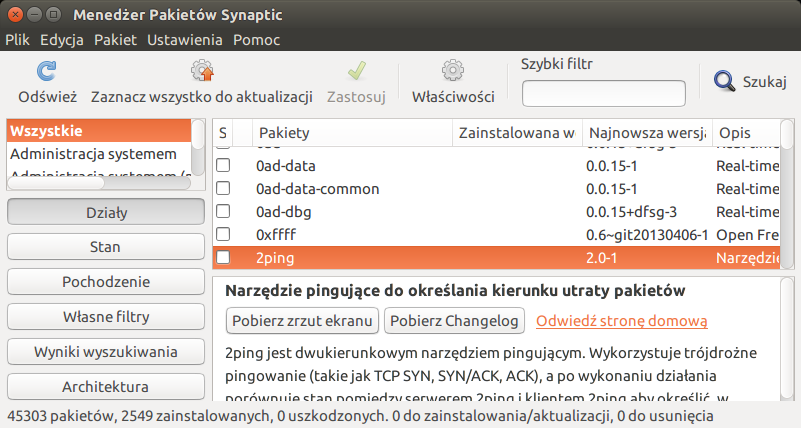
\includegraphics[width=\linewidth]{images/programy_synaptic.png}
\end{center}

\subsubsection{Instalacja programów w konsoli}
Graficzne narzędzia są wygodne, ale czasem trzeba sięgnąć po konsolę. Często na forach pomocy technicznej właśnie ten sposób jest przedstawiany podczas metod rozwiązywania problemów. Jedno polecenie w konsoli łatwiej wstukać niż opisywać jak przedostać się przez gąszcz przycisków i menusów. Wynika to z założenia, że nie każdy musi mieć zainstalowany Menadżer pakietów. Nawet Centrum Oprogramowania może być nieobecne w systemie - to program jak każdy inny i może zostać usunięty.
W dalszych częściach tego Przewodnika kilkukrotnie przedstawiamy instalację paczek właśnie w ten sposób.

Konsolowym menadżerem pakietów w systemie Ubuntu jest \textcolor{ubuntu_orange}{apt-get}. Ma on takie same możliwości jak opisywany wcześniej Synaptic, z tym że polecenia wydaje się klawiaturą a nie myszą. Aby zainstalować pakiet z oprogramowaniem przy pomocy apt-get:
\begin{enumerate}
\item Uruchom konsolę, wpisując w Dashu \textcolor{ubuntu_orange}{Terminal} lub wciskając kombinację klawiszy \keys{CTRL + Alt + t}.
\item Wpisz:
\begin{lstlisting}[language=bash]
sudo apt-get install vlc
\end{lstlisting}
\item Wciśnij \keys{\returnwin}
\item wpisz swoje hasło i wciśnij \keys{\returnwin}. nie przejmuj się, że hasło się nie pojawia. Jest to zabezpieczenie przed podglądaczami.
\end{enumerate}
VLC jest znanym na całym świecie kombajnem do odtwarzania wszelkiego rodzaju multimediów. Nie ma go w standardowej instalacji Ubuntu, ale dostępny jest za pośrednictwem repozytoriów. Co oznaczają poszczególne części tego polecenia?
\begin{itemize}
\item \textcolor{ubuntu_orange}{sudo} --- instalacja pakietów (a także ich usuwanie) wymaga uwierzytelnienia i tylko administrator systemu może to zrobić. \textit{Sudo} jest programem umożliwiającym wykonanie kolejnego polecenia jako inny użytkownik (w tym wypadku root, administrator). Spróbuj wpisać to polecenie bez sudo z początku i zobacz co się stanie.
\item \textcolor{ubuntu_orange}{apt-get} --- to konsolowy program do zarządzania pakietami.
\item \textcolor{ubuntu_orange}{install} --- opcja \textit{install} jest jedną z możliwości programu apt-get. W tym wypadku każe mu wykonać instalacje programu.
\item \textcolor{ubuntu_orange}{vlc} --- jaki program chcemy zainstalować. Zwróć uwagę, że nazwy programów pisane są zawsze małymi literami, a także podawane są bez rozszerzenia.
\end{itemize}

Po podaniu hasła apt-get przetworzy żądanie (zainstaluj pakiet vlc) i wyświetli informacje podobną do poniższej:

\begin{lstlisting}[language=bash]
Czytanie list pakietów... Gotowe
Budowanie drzewa zależności       
Odczyt informacji o stanie... Gotowe
Zostaną zainstalowane następujące dodatkowe pakiety:
  libbasicusageenvironment0 libcddb2 libcrystalhd3 libdvbpsi8 libebml4 libgnutls28 libgroupsock1 libhogweed2 libiso9660-8 liblivemedia23 libmatroska6
  libproxy-tools libresid-builder0c2a libsdl-image1.2 libsidplay2 libssh2-1 libtar0 libupnp6 libusageenvironment1 libva-x11-1 libvcdinfo0 libvlc5
  libvlccore7 libxcb-composite0 libxcb-keysyms1 libxcb-xv0 vlc-data vlc-nox vlc-plugin-notify vlc-plugin-pulse
Sugerowane pakiety:
  firmware-crystalhd gnutls-bin videolan-doc
Polecane pakiety:
  libdvdcss2
Zostaną zainstalowane następujące NOWE pakiety:
  libbasicusageenvironment0 libcddb2 libcrystalhd3 libdvbpsi8 libebml4 libgnutls28 libgroupsock1 libhogweed2 libiso9660-8 liblivemedia23 libmatroska6
  libproxy-tools libresid-builder0c2a libsdl-image1.2 libsidplay2 libssh2-1 libtar0 libupnp6 libusageenvironment1 libva-x11-1 libvcdinfo0 libvlc5
  libvlccore7 libxcb-composite0 libxcb-keysyms1 libxcb-xv0 vlc vlc-data vlc-nox vlc-plugin-notify vlc-plugin-pulse
0 aktualizowanych, 31 nowo instalowanych, 0 usuwanych i 0 nieaktualizowanych.
Konieczne pobranie 10,4 MB archiwów.
Po tej operacji zostanie dodatkowo użyte 51,3 MB miejsca na dysku.
Kontynuować? [T/n] 
\end{lstlisting}

To duże tekstu, ale bardzo łatwo go zinterpretować:

\begin{itemize}
\item \textcolor{ubuntu_orange}{Czytanie list pakietów... Gotowe} --- apt-get przetworzył bazę danych pakietów i znalazł na liście program VLC
\item \textcolor{ubuntu_orange}{Budowanie drzewa zależności} --- apt-get sprawdził jakich innych pakietów VLC.
\item \textcolor{ubuntu_orange}{Zostaną zainstalowane następujące dodatkowe pakiety:} --- Lista pakietów, które muszą być zainstalowane razem z VLC aby ten mógł działać.
\item \textcolor{ubuntu_orange}{Sugerowane pakiety:} --- lista przydatnych pakietów, które nie zostaną teraz zainstalowane ale mogą się kiedyś przydać.
\item \textcolor{ubuntu_orange}{Polecane pakiety:} --- podobnie jak sugerowane pakiety, ale z większym naciskiem na ich przydatność. W tym wypadki apt-get zaproponował instalację biblioteki umożliwiającej odtwarzanie zaszyfrowanych płyt DVD. jeżeli podążasz zgodnie z tym Przewodnikiem, ta paczka została omówiona w rozdziale \ref{ubuntu-restricted-extras}
\item \textcolor{ubuntu_orange}{Zostaną zainstalowane następujące NOWE pakiety:} --- lista wszystkich pakietów, które zostaną zainstalowane. Automatyczna instalacja sugerowanych i polecanych pakietów domyślnie jest wyłączona.
\item \textcolor{ubuntu_orange}{0 aktualizowanych, 31 nowo instalowanych, 0 usuwanych i 0 nieaktualizowanych.} --- podsumowanie. Niektóre paczki są w konflikcie ze sobą (np. różne wersje tego samego programu) i instalacja jednej wymusza odinstalowanie innej.
\item \textcolor{ubuntu_orange}{Konieczne pobranie 10,4 MB archiwów.} --- ile danych zostanie pobranych z internetu.
\item \textcolor{ubuntu_orange}{Po tej operacji zostanie dodatkowo użyte 51,3 MB miejsca na dysku.} --- ile miejsca zostanie zajęte po tej operacyji.
\item \textcolor{ubuntu_orange}{Kontynuować? [T/n]} --- wciśnij \keys{t} aby rozpocząć pobieranie i instalację, lub \keys{n} aby przerwać procedurę.
\end{itemize}

Apt-get pobierze teraz wszystkie paczki, sprawdzi ich spójność (sumy kontrole oraz podpisy cyfrowe), rozpakuje je w systemie plików zgodnie z instrukcjami zawartymi w paczce i skonfiguruje zainstalowane programy (np. poinformuje menadżer plików, że teraz filmy ma odtwarzać w VLC a nie w domyślnie zainstalowanym Totemie).

Inne opcje programu apt-get to:

\begin{itemize}
\item \textcolor{ubuntu_orange}{update} --- pobiera z serwerów repozytoriów najświeższą listę pakietów.
\item \textcolor{ubuntu_orange}{upgrade} --- aktualizuje wszystkie zainstalowane pakiety.
\item \textcolor{ubuntu_orange}{dist-upgrade} --- aktualizuje wszystkie zainstalowane pakiety a także dokonuje instalacji nowych pakietów wskazanych przez aktualizacje (lub usuwa już niepotrzebne).
\item \textcolor{ubuntu_orange}{check} --- sprawdza stan zainstalowanych pakietów. Wyświetli informacje, jeżeli czegoś brakuje lub jakieś paczki są niepotrzebne.
\item \textcolor{ubuntu_orange}{remove} --- usuwa z systemu wskazaną paczkę.
\item \textcolor{ubuntu_orange}{purge} --- usuwa z systemu wskazaną paczkę wraz z pozostałościami (pliki konfiguracyjne, dokumentacja, logi itp.)
\end{itemize}

\subsubsection{Instalacja dodatkowych repozytoriów}
W skład standardowych repozytoriów Ubuntu wchodzi około 45 tysięcy paczek. Liczba ta wydaje się ogromna, ale jest to jedynie ułamek dostępnego oprogramowania. Te 45 tysięcy pakietów jest zarządzanych i sprawdzanych przez Canonicala i nie ma możliwości aby dbali oni o każdy, najmniejszy program. Dlatego w ręce deweloperów aplikacji został oddany mechanizm PPA. Najczęściej zarejestrowanie takiego PPA opisywane jest jako szereg trzech komend, które trzeba wydać w terminalu. W tym przykładzie zarejestrujemy PPA należące do pakietu biurowego LibreOffice. W tym repozytorium znajdują się aktualizacje tego zestawu programów, które nie trafiły na serwery Canonical
\begin{enumerate}
\item Dodaj repozytorium:
\begin{lstlisting}[language=bash]
sudo apt-add-repository ppa:libreoffice/ppa
\end{lstlisting}
Przy każdym dodawanym PPA program wyświetli skrócone informacje. Zapoznaj się z nimi i wiciśnij \keys{\returnwin} aby dodać to repozytorium do systemu lub \keys{ctrl + c} aby przerwać operację.
\item Zaktualizuj listę pakietów
\begin{lstlisting}[language=bash]
sudo apt-get update
\end{lstlisting}
\item Zainstaluj LibreOffice
\begin{lstlisting}[language=bash]
udo apt-get install libreoffice
\end{lstlisting}
\end{enumerate}

Aby dodać repozytorium w sposób graficzny wykonaj następujące czynności:
\begin{enumerate}
\item W dashu uruchom \textcolor{ubuntu_orange}{Oprogramowanie i Aktualizacje}.
\item Przejdź do zakłądki \textcolor{ubuntu_orange}{Inne oprogramowanie}.
\item Kliknij przycisk \textcolor{ubuntu_orange}{Dodaj}
\item W pole \textcolor{ubuntu_orange}{Wiersz APT} wpisz adres repozytorium, tutaj: \textit{ppa:libreoffice/ppa}
\item Kliknij \textcolor{ubuntu_orange}{Dodaj zasób} a nastepnie \textcolor{ubuntu_orange}{Zamknij}
\item Zostaniesz poproszony o zaktualizowanie listy pakietów. Wykonaj tę czynność.
\end{enumerate}

\subsubsection{Instalacja pakietów .deb}
Niektórzy twórcy programów nie opiekują się własnymi repozytoriami, ale zamiast tego przygotowują paczki z oprogramowaniem do ręcznej instalacji. Takie paczki mają rozszerzenie \textit{.deb}. Identyczne paczki sa pobierane z repozytoriów za pomocą Centrum Oprogramowania, Synaptica albo apt-get, z tym że proces rozwiązywania zależności jest przez te programy prowadzany automatycznie, zaś przy ręcznej instalacji paczek .deb nie.

Aby zainstalować pobraną paczkę .deb masz dwie możliwości. W konsoli:
\begin{lstlisting}[language=bash]
sudo dpkg -i nazwa_paczki.deb
\end{lstlisting}
\begin{itemize}
\item \textcolor{ubuntu_orange}{sudo} --- instalacja pakietów (a także ich usuwanie) wymaga uwierzytelnienia i tylko administrator systemu może to zrobić.
\item \textcolor{ubuntu_orange}{dpkg} --- to konsolowy program do zarządzania paczkami .deb
\item \textcolor{ubuntu_orange}{-i} --- flaga dla programu dpkg informująca go, że ma zainstalować wskazaną paczkę.
\item \textcolor{ubuntu_orange}{nazwa\_paczki.deb} --- wskazujesz na wcześniej pobraną paczkę.
\end{itemize}

Po takiej operacji raczej na pewno otrzymasz komunikat o ,,niespełnionych zależnościach''. Dpkg nie pobierze i nie zainstaluje brakujących pakietów. Na szczęście apt-get potrafi to naprawić. Wykonaj:
\begin{lstlisting}[language=bash]
sudo apt-get install -f
\end{lstlisting}
Opcja \textcolor{ubuntu_orange}{install} z flagą \textcolor{ubuntu_orange}{-f} informuje apt-get, że ma sprawdzić stan paczek oraz zreperować (f czyli fix) stan pakietów. Po tej operacji program zostanie prawidłowo zainstalowany i skonfigurowany, a paczkę .deb można skasować.

Aby graficznie zainstalować pobraną paczkę deb potrzebujesz odpowiedniego programu. Nazywa się on \textcolor{ubuntu_orange}{GDebi}. Znajdziesz go w Centrum oprogramowania, Synapticu lub zainstalujesz z konsoli poleceniem
\begin{lstlisting}[language=bash]
sudo apt-get install gdebi
\end{lstlisting}

Kiedy GDebi jest gotowy do użycia kliknij prawym przyciskiem myszy na paczkę deb a następnie wybierz \menu{{Otwórz za pomocą}>{GDebi Package Installer}}. Teraz wystarczy kliknąć \textcolor{ubuntu_orange}{Install} aby GDebi sprawdził zależności i zainstalował wszystko co potrzeba.

\subsubsection{Instalacja programów .bin}
Niektórzy dostawcy oprogramowania (na szczęście nieliczni) udostępniają własne instalatory programów, na sposób znany z systemu Windows (pliki .exe i .msi). Na szczęście są to coraz rzadsze przypadki. Jednak gdybyś przypadkiem trafił na tak przestarzały sposób dystrybucji programu to kliknij prawym przyciskiem myszy na pobranym programie i wybierz \menu{{Właściwości}>{Uprawienia}>{Wykonywanie}} i zaznacz pole \textcolor{ubuntu_orange}{Zezwolenie na wykonywanie pliku jako programu}. Teraz kliknij dwukrotnie lewym przyciskiem myszy na pliku aby go uruchomić.

\subsubsection{Instalacja programów przez przeglądarkę internetową}
Przeglądarka internetowa Firefox wchodząca w skład standardowej instalacji Ubuntu wyposażona jest w dodatek umożliwiający instalacje oprogramowania bezpośrednio ze strony internetowej poprzez protokół apt. Kliknięcie na odpowiedni link otworzy okno \textcolor{ubuntu_orange}{Centrum Oprogramowania Ubuntu} na stronie danego programu.

Jeżeli Firefox nie rozpoznaje protokołu apt to wyświetli okno z prośbą o wybór aplikacji. Kliknij na przycisk \textcolor{ubuntu_orange}{Wybierz\ldots} a następnie wskaż plik \menu{{System plików}>{usr}>{bin}>{software-center}}. Pamiętaj aby zaznaczyć pole \textcolor{ubuntu_orange}{Zapamiętaj wybór dla odnośników apt}.
